%!TEX root = paper.
\begin{figure*}[!t]
\begin{minipage}{0.310\linewidth}
  \centering
  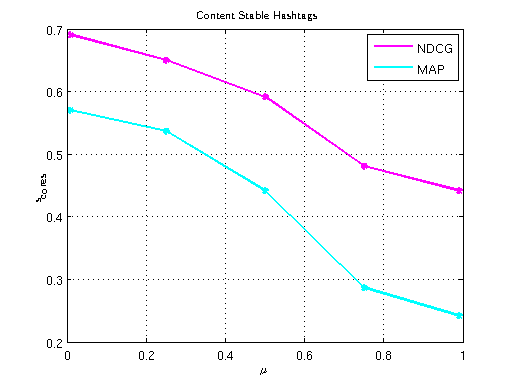
\includegraphics[width=1\textwidth]{KDD/images/content}             
   (a) content stable; $k = 5$ 
\end{minipage}
\begin{minipage}{0.310\linewidth}
  \centering
  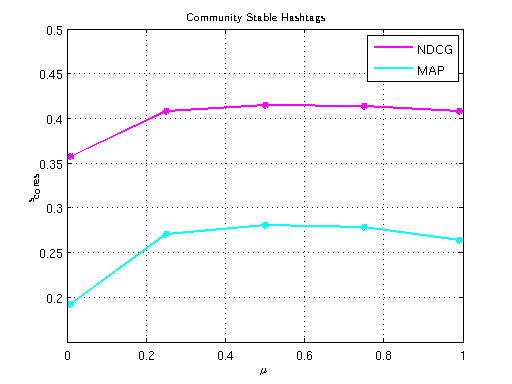
\includegraphics[width=1\textwidth]{KDD/images/community}             
  (b) community stable; $k = 5$
\end{minipage}
\begin{minipage}{0.310\linewidth}
  \centering
  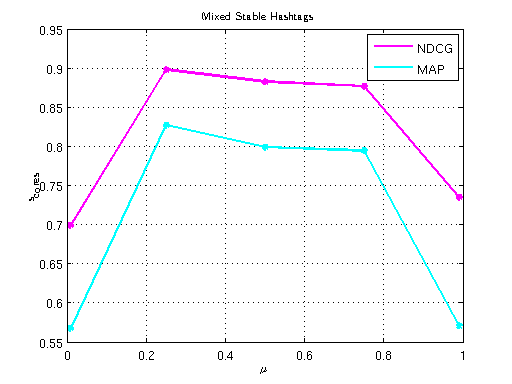
\includegraphics[width=1\textwidth]{KDD/images/mixed}             
  (c) mixed stable; $k = 5$
\end{minipage} \\
\begin{minipage}{0.310\linewidth}
  \centering
  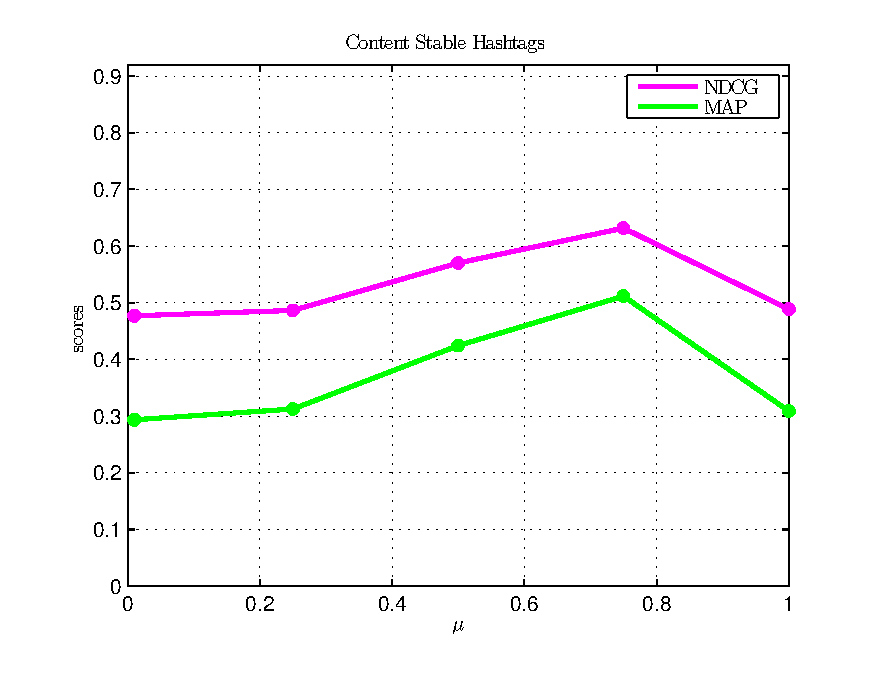
\includegraphics[width=1\textwidth]{KDD/images/content_t_15}             
   (d) content stable; $k = 15$
\end{minipage}
\begin{minipage}{0.310\linewidth}
  \centering
  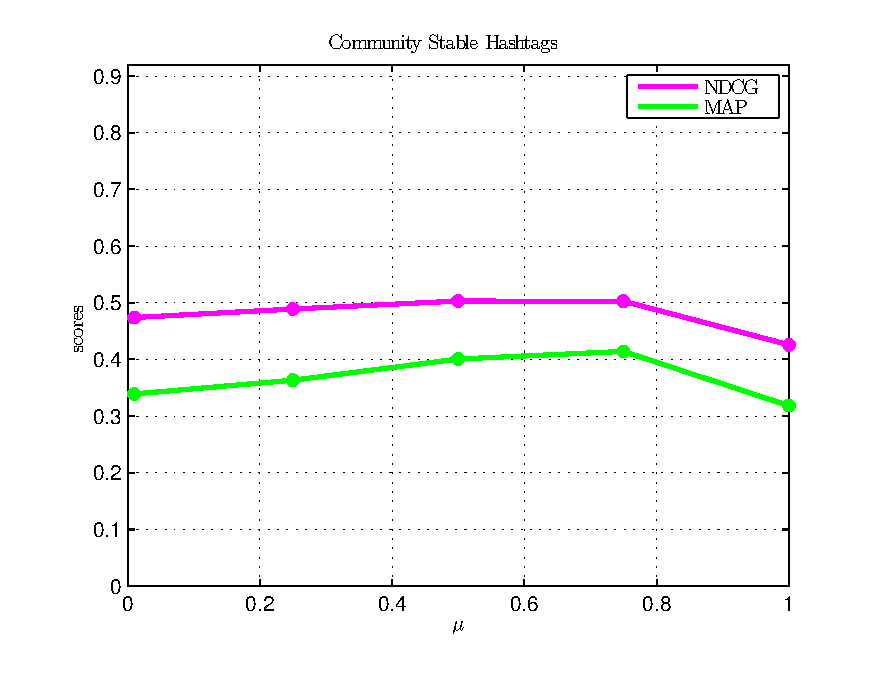
\includegraphics[width=1\textwidth]{KDD/images/community_t_15}             
  (e) community stable; $k = 15$
\end{minipage}
\begin{minipage}{0.310\linewidth}
  \centering
  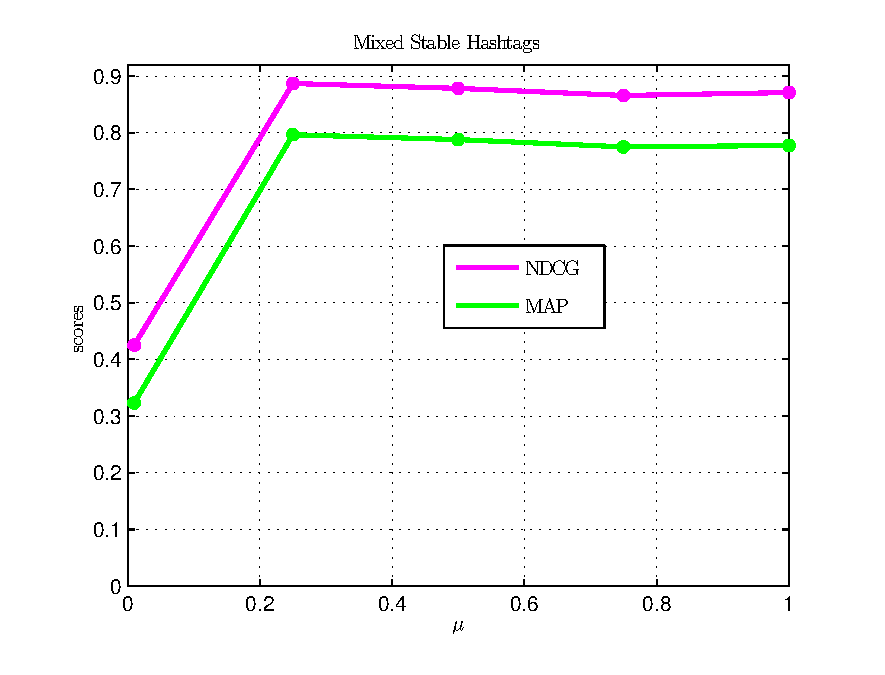
\includegraphics[width=1\textwidth]{KDD/images/mixed_t_15}             
  (f) mixed stable; $k = 15$
\end{minipage}
  \caption[Effect of $\mu$.]{{This figure illustrates the effect of the importance parameter, $\mu$ on the performance.  
Refer to Equation \ref{eq:loss_function}.  A high value of $\mu$ places more weight on the topic part of the objective
and less weight on the community part of the objective, and vice versa.
}}
\label{fig:mu_analysis}
\end{figure*}
Recall that our goal in this work is to gain a better understanding of when the
social context surrounding the documents actually improve topic discovery.
Hence, in this section, our primary focus is to provide a quantitative and 
qualitative answers to each of the research questions posed in the introduction. 
Section \ref{subsec:baselines} provides an overview about the baseline algorithms,
details how we implement them, and how we use them in our
problem setting.  Section \ref{subsec:ground_truth_evaluation}
provides details about how the groundtruth topics are obtained.  In addition,
it also explains how the topics detected by our algorithm and each of the baselines are compared with
the groundtruth  topics, and what metrics are used for the evaluations.
Then, each of the subsequent subsections are dedicated to answering one or more 
research questions.
\subsection{Baselines}
\label{subsec:baselines}
We evaluate our algorithm with several baselines.  Our baselines can be divided into two categories;
one which focuses on modeling topic evolution, and another which aims to incorporate link information
into topic modeling.

\emph{Link-PLSA-LDA} \cite{Nallapati:2008} is an algorithm which uses both the content
and link information (but does not have a temporal aspect incorporated in it). 
The link structure is built from the citation network of the documents.
The algorithm combines LDA and PLSA into a single
framework and in addition, models the topical relationship between the citing document
and the cited document.\footnote{While we do not explicitly compare to \cite{Erosheva:2004}, the
authors of Link-PLSA-LDA compare
their own work to former and claim better performance.}  The inference is carried out by
employing mean-variation approximation of the latent variables.  To implement this algorithm, 
we used the code developed by the authors which is available publicly.\footnote{\hyperref[]{https://sites.google.com/site/rameshnallapati/software}}  As input, the algorithm requires
a list of documents in a bag-of-words format, and a matrix of links between the documents.  Producing
bag-of-words for each document is straightforward.  For the link information, 
we assume that a link exists between two articles if they have a common user sharing or posting
the article.  This information was essentially derived from the $\mathbf{U}$ matrix in Section
\ref{sec:data_set_description}.  Each fresh inflow of documents is considered as a separate problem
as the model was not developed to connect topics temporally.

\emph{Collective Matrix Factorixation} (CMF) \cite{Saveski:2014, Ding:2014} 
Broadly speaking, the concept of collective matrix factorization has been
used in several applications including recommendation systems, producing hashing functions for images, co-clustering etc.
In this scenario, we will use CMF to incorporate both the social and textual aspect
of the objective in Equation \ref{eq:loss_function} but not its temporal aspect.
We compare our method to this
baseline to show that using the temporal information of tracking the textual content and community helps improve
performance.

\emph{Online-LDA} \cite{AlSumait:2008} is an algorithm which monitors topic evolution, in that it utilizes 
the information about topics detected in the previous time steps, but does not accommodate 
for the link structure between the documents.  We implemented Online-LDA based
on the original LDA code developed by David Blei\footnote{\hyperref[]{http://www.cs.princeton.edu/~blei/lda-c/}} 
(as suggested by the authors of \cite{AlSumait:2008}).  The authors
of \cite{AlSumait:2008} had found that using the topics detected in the previous time step produced the most improvement in
performance, and suggested that using the topics from earlier time steps produced only marginal improvements.  
We tested this baseline in a similar setting as well and used only the topics in the previous timestep to discover current topics.
In essense, implementing Online-LDA boils down to setting the prior on the topics according to the topic
distribution discovered in the previous time step.

\emph{Joint Past Present Decomposition} (JPP) \cite{Vaca:2014} models also the topic evolution, but as Online-LDA, is blind to the social context surrounding the  input documents.  Our method, LTECS, reduces to JPP when $\mu = 1$.
We used the code provided by the authors.\footnote{\hyperref[]{https://github.com/amantrac/TopicDiscoveryJPP}}
\subsection{Evaluation, Groundtruth and Experimental Setup}
\label{subsec:ground_truth_evaluation}
We evaluate all the algorithms by comparing a ranking of the top-$10$ words obtained by each
algorithm, and a ranking of the top-$10$ words obtained by the groundtruth.  It has been shown that
the group of top-$10$ words indeed give us a good insight about the topic \cite{sekiguchi:2006,newman2010automatic}.
All the algorithms considered here including the baselines and LTECS
discover topics by directly producing a distribution over words. 
In terms of mapping the discovered topics to the groundtruth topics, we calculated
the cosine similarity between each of the discovered topics and the groundtruth topics.
Each discovered topic was then mapped to the most similar groundtruth topic.
We borrow this procedure procedure from other state of the art experiments
in topic evolution \cite{Saha:2012}.
The distributions produced in each case are discrete and can be used 
to pick the top-$10$ words in each topic and to produce a ranking.

We now delve a bit more into how the groundtruth is obtained.  On Twitter, hashtags are a sequence of non-whitespace
characters which follow the \# sign.  It is popular convention on Twitter to embed a hashtag
in a tweet to give it context.
And as in several studies in the past, this context is used as the groundtruth topic annotations for
the news articles whose links are embedded in the tweet \cite{Tsur:2012}. 
The hashtags for each of the three categories, content stable,
community stable, and mixed stable were identified as explained in Section \ref{subsec:hashtag_stability}.

The way we calculate
the actual groundtruth topic distribution is that, 
at each time step, the $\mathbf{T}^{(t)}$
matrix (refer to Section \ref{sec:data_set_description} for notation) is premultiplied by $\mathbf{X}^{(t)}$
to obtain a resulting matrix of raw word counts for each topic.  Premultiplication of $\mathbf{T}^{(t)}$
by $\mathbf{X}^{(t)}$ basically yields the average word distribution within each hashtag.  
Once this is obtained, the highest weighted $10$ words form our groundtruth ranking.  We use
Normalized Cumulative Discounted Gain (NDCG) metric, and the Mean Average Precision (MAP) metric
to compare the rankings obtained by each algorithm to the groundtruth.  We have performed
experiments by considering the best $5,10,15 \text{ and } 20$ topics for each category.  

We now give details about the experimental setup.  Our objective function is optimized
iteratively using the multiplicative update equations (Equations \ref{eq:W_update} - \ref{eq:MC_update})
in Section \ref{sec:content_and_networks}.  The variables $\W, \HH, \G, \MT, \MC$ were given
a random non-negative initialization.  The parameters were tuned on all
the data.  In both datasets, the data spans for 14 days, and hence the topic discovery results that
we obtained are averages of the results obtained over that time period.
The $l1$ normalization parameter for CMF, the JPP model and the LTECS model were set to $0.05$.
The $\lambda$ parameter was tuned for values of $\{10, 100, 10^3 \ldots 10^7\}$.  It was consistently
observed that the algorithm yielded good performance for $\lambda = 10^7$
\footnote{While it so happens that this value of lambda worked well for the Twitter dataset, it may
not hold for other datasets.  As a matter of fact, we explore this more in Section \ref{subsec:learning_stability}
where we try to assess the quality of topics by setting $\alpha = 0.5$ and $\lambda = 0$.}.
We tuned for different values of $\mu \in \{0.01, 0.25, 0.5, 0.75, 1\}$ and picked the one which gives the best performance.
We delve more into the analysis for $\mu$ in subsequent sections.  For the baselines, all the parameters
were tuned and set internally.
\subsection{Social Information Vs Textual Content: the Trade-off}
\label{subsec:parameter_analysis}
The $\mu$ parameter from Equation \ref{eq:loss_function} allows to
bias the objective function more
towards one of the modalities, if so desired.  A high value of $\mu$ biases importance to the content part of
the objective and vice versa.  In fact, LTECS reduces to JPP when $\mu = 1$ and hence JPP can never
outperform LTECS.  This section delves into investigating how the trade-off between using content and social information
actually functions on both datasets. 

For the case of \emph{community stable} hashtags, the best performances
were achieved for $0.01 \leq \mu \leq 0.5$ (Table \ref{tab:topic_discovery_evaluation}).
This implies that when a lot of importance was placed on the social context part
of the objective, better were the topics that were detected. Refer to Figure \ref{fig:mu_analysis}b
and \ref{fig:mu_analysis}e.  These figures illustrate how the performance varies as the value of $\mu$
moves from $0$ to $1$.  Note that highest performance is achieved when $\mu \leq 0.5$.

While considering \emph{content stable} hashtags, we will focus on LTECS and JPP
in Table \ref{tab:topic_discovery_evaluation}. For $k = 5 \text{ and } 10$, we observe best
performances by \emph{both} JPP and LTECS method.  In other words, LTECS
algorithm exhibited best performance when the objective contained only the content part with $\mu = 1$.  
This suggests that for topics which have a highly focused text, we need to place all the 
importance on content.  What is more interesting is that, it implies that even if we add a little
bit of the social context information to the objective, it actually \emph{hurts} performance.
Let us contrast this result to what happens when $k = 15 \text{ and } 20$.
In those scenarios, we observe that the best performance was
obtained by LTECS, when $\mu$ was $0.75$.  
For the purest $5$ and $10$ topics, it could be that the content of those documents 
were very well defined that the usage of side information actually detracted the objective 
from the correct path.  However as the number of topics
increases ($k = 15, 20$), there is perhaps more noise in the topics and
we find that the use of community information indeed helps.  
This suggests that for the best performance one needs to know the accurate
operating spot of the $\mu$ parameter.  
The important message from analyzing the $\mu$ trade-off for content stable and community
stable hashtags is that, with very focused text, just using the content suffices. This is likely to be the case for the dominant topics (i.e. $k<10$ in our study).
On the other hand, if the text is a little noisy, the social context greatly
helps in discovering better topics. 
This is likely to be the case when tracking more than just the top dominant topics ($k>10$ in our case).  
As we argue in the introduction, in today's world,
the text is more often than not quite noisy as topics are prone to being volatile and evolving
very quickly.  Refer to Figures \ref{fig:mu_analysis}(a) and \ref{fig:mu_analysis}(d).  The figure
illustrates that the best performance is acheived when $\mu \geq 0.5$.

By definition \emph{mixed stable} hashtags have both stable content and stable communities.  
As it turns out, the best performance for LTECS is obtained when $0.25 \leq \mu \leq 0.75$.
This suggests that when we have topics which have both stable content and community,
it is necessary to give importance to both aspects.  In addition, biasing only on content
does not yield the best performance.  In Figures \ref{fig:mu_analysis}(c) and \ref{fig:mu_analysis}(f),
the best performance is achieved in the midregion of the plot.
\subsection{Comparison with the state-of-the-art}
\label{subsec:topic_discovery_experiments}
In this section, we discuss how our algorithm performs in 
comparison to state of the art baselines introduced in Section \ref{subsec:baselines}.
One of the main conclusions from analyzing the results is that, using the community
information certainly helps with better topic tracking.  This is a direct observation
from Table \ref{tab:topic_discovery_evaluation} that the NDCG and MAP values for LTECS
is higher, or at least as good as its competitors in most scenarios.  The rest of this section
will highlight where the sweet spot of the trade off between content and community
lies, and why.

For \emph{community stable topics}, as expected, good improvements were seen in the community stable hashtags.  In these hashtags,
LTECS algorithm consistently outperforms all the baselines.  It is clear that
the use of community information helps in better topic discovery.  It is also interesting
to note that the algorithm that exhibits second best performance is Link-PLSA-LDA.  
Hence, not learning from older topics does not particularly hurt Link-PLSA-LDA
in its performance when compared to Online-LDA and JPP.  This means that, for community stable topics, 
the algorithms that use some form
of social context information or link information perform better than those that discover topics using
content alone.

In the case of \emph{content stable topics}, one may expect the baselines which focus only
on the content of the documents to exhibit best performance.  This is partially true.  For $k = 5,10$,
JPP and LTECS outperform Link-PLSA-LDA and Online-LDA.  Note that in both cases
LTECS achieves the best performance only when $\mu = 1$ implying that adding community information
does not help.  On the other hand, for $k = 15 \text{ and } 20$, LTECS achieves best performance
over all the baselines.  In these cases note that the value for $\mu = 0.75$.  This implies
that adding the community information actually helps.  We already discussed this behavior in Section \ref{subsec:parameter_analysis}.
 Another thing to note here is that Link-PLSA-LDA some what consistently ranks last.  This is because
Link-PLSA-LDA, unlike LTECS lacks the tuning parameter $\mu$ which can seamlessly shift the focus of the
objective between topic and community.  It perhaps places equal weight on both, and hence fails to
make the appropriate tradeoff.

For \emph{mixed stable hashtags}, the performance is in generally very good for all the hashtags.
This becomes clear when we compare the performance metrics of content stable and community stable to mixed stable.  There
is a noticeable jump in the average NDCG and MAP scores.  This implies that, if a hashtag
has both well focused content, and a dedicated community of users, detecting those topics
are much easier. 
\begin{table*}[!t]
\begin{center}
{\small 
{\renewcommand{\arraystretch}{0.91}
\begin{tabular}{||c|c|c|cccc||}
\hline
 Category of Topic &Metric & Model & k = 5 & k = 10 & k = 15 & k = 20\\
\hline
 		    & & LTECS & 0.4081 & \textbf{0.4800} & \textbf{0.5029} & 0.5129\\
Community 	& &  & $\mu =  0.01$  & $\mu = 0.5$ & $\mu =  0.5 $ & $\mu = 0.5$\\ \cline{4-7}	
		    & NDCG & JPP & 0.3699 & 0.4496 & 0.4608 &0.4138\\
			&  & Online-LDA & 0.3903 & 0.4138 &0.4446  & 0.5667 \\
Stable       & & Link-PLSA-LDA &0.3943 & 0.4608 & 0.4761 & 0.4925\\ 
        & & CMF & 0.3454 & 0.4338 & 0.4771 & 0.4827 \\ \cline{4-7}
		& & LTECS & 0.2653 & 0.3637 & \textbf{0.4007} & \textbf{0.4173}  \\
		& &  &$\mu = 0.01$ & $\mu = 0.5 $ & $\mu = 0.5$  & $\mu = 0.5$ \\ \cline{4-7}
Hashtags&MAP & JPP &  0.2191 & 0.3596 & 0.3462 & 0.3420 \\
		& & Online-LDA & 0.2628  & 0.3160 & 0.3489 & 0.3835 \\
		& & Link-PLSA-LDA & 0.2704 & 0.3364  & 0.3658 & 0.3937 \\
        & & CMF & 0.2044 & 0.3190 & 0.3757 & 0.3665 \\
\hline
		& & LTECS &\ 0.6888 & 0.6055& \textbf{0.6317}& \textbf{0.6623} \\
Content   & &  & $\mu =  1$  & $\mu = 1$ & $\mu =  0.75 $ & $\mu = 0.75$\\ \cline{4-7}
		&NDCG & JPP & 0.6888 & 0.6055 &  0.4885&  0.6504 \\
		& & Online-LDA & 0.6815& 0.5988 & 0.6166 & 0.6684  \\
Stable  & & Link-PLSA-LDA & 0.6574 & 0.5862 & 0.6087& 0.6401\\ 
        & & CMF & 0.5846 & 0.4919 & 0.4455 & 0.4327 \\\cline{2-7}
		& & LTECS & \textbf{0.5655} &  \textbf{0.4784}& \textbf{0.5115} & \textbf{0.5559}  \\
		& &  & $\mu =  1$  & $\mu = 1$ & $\mu =  0.75$ & $\mu = 0.75$\\ \cline{4-7}
Hashtags &MAP & JPP &  0.5655 & 0.4784 & 0.3089 & 0.5411  \\
		& & Online-LDA &  0.5175 & 0.4083 & 0.4555 & 0.5443 \\
		& & Link-PLSA-LDA & 0.4890 & 0.3817  &0.4434 &0.5053  \\
        & & CMF & 0.4423 & 0.3207 & 0.2556 & 0.2557 \\
\hline
	    & & LTECS & 0.9005 & 0.8868& \textbf{0.9249}& 0.9089 \\
Mixed   & &  & $\mu =  0.25$  & $\mu = 0.75$ & $\mu =  0.25 $ & $\mu = 0.25$ \\ \cline{4-7}
		&NDCG & JPP & 0.8771 & 0.8762 & 0.4251 & 0.4580 \\ 
	    & & Online-LDA &\textbf{0.9564} & 0.9168 & 0.9111 & 0.5967 \\
Stable  & & Link-PLSA-LDA & 0.8944 & 0.9159 &0.8392 & 0.8975 \\ 
        & & CMF & 0.6712 & 0.8768 & 0.8905 & 0.8753 \\ \cline{2-7}
		& & LTECS & 0.7783 &0.7965  & \textbf{0.8964} & 0.8845 \\
		& &  & $\mu =  0.25$  & $\mu = 0.75$ & $\mu =  0.5$ & $\mu = 0.25$ \\ \cline{4-7}
Hashtags&MAP & JPP &  0.7762 & 0. 7783 & 0.3232 & 0.3644  \\ 
		& & Online-LDA & \textbf{0.9208}  & \textbf{0.8804} & 0.8841 & 0.4308 \\
		& & Link-PLSA-LDA & 0.8787 & 0.8379  & 0.7452 & \textbf{0.8982} \\
        & & CMF & 0.5329 & 0.8223 & 0.8499 & 0.8337 \\
\hline
\end{tabular}
}
}
\caption[Evaluation of topic discovery]{{Topic discovery evaluation using Normalized Cumulative Discounted Gain and Mean Average Precision metrics
for all three categories of hashtags.  $k$ stands for the number of topics.  $\lambda$ was set to $10^7$, and $\alpha$ was set to 0.05 for LTECS model.
All the values in bold represent significant improvement in performance (using Student-t test, $p < 0.05$).}}
\label{tab:topic_discovery_evaluation}
\end{center}
\end{table*}
\subsection{Learning Stability of Topics}
\label{subsec:learning_stability}
In this section, we investigate to what extent can our algorithm learn the type of
topics present in the documents; i.e., are the documents more content stable,
community stable or mixed stable. And we certainly do not want to be able to bias the
objective function more towards one of the modalities.  Hence, for all experiments
in this section, we set $\mu = 0.5$.
Recall that our loss function (Equation \ref{eq:loss_function}) is built such
that $\HH \approx \mathbf{M} \Htt$. 
The proposed model encourages for stability of topics and communities by regularizing the evolution matrices 
$\MT$ and $\MC$
through $\lambda(||\MT - \I||_F^{2} + ||\MC - \I||_F^2)$. 
A high value of $\lambda$ pushes the evolution matrices close to $\mathbf{I}$ 
which enforces the topics (and communities) to evolve very little over time.  
So far, we demonstrated the effectiveness of using side social information in 
order to discover topics on large scale dataset based on Twitter.
In this section, we aim to assess the extent to which our 
algorithm is able to recover correctly the evolution patterns exhibited by 
the data by studying the evolution matrices $\MT$ and $\MC$ across consecutive time steps.

This raises the question of how to set $\lambda$. In presence of a groundtruth this parameter 
can be tuned by cross validation as we did in the previous section (where hashtags where used as proxy 
to build the groundtruth). However, in the real world, topical annotations are rarely available. 
In this context, the user can decide to use the model in an ``agnostic mode" by not placing 
any form of prior on the evolution matrices. 
This is achieved by setting $\lambda$ to 0.  In this real world scenario, we may wonder if the model, 
without the help of any prior, will be able to recover the correct evolution patterns. In other words, we 
propose to test the extent to which the retrieved evolution matrices are close to the ``real ones". To do so, 
we make use of the group of hashtags previously identified (Section \ref{sec:data_set_description}) as 
stable and unstable at the topic and community level. To validate that the retrieved $\mathbf{M}$ 
matrices exhibit a temporal stability pattern which is indeed present in the data, we test if the matrix retrieved 
from the stable group of hashtags is closer to the identity than the one retrieved from 
the unstable group (for both topics and communities).  In other words, for topic stable hashtags,
we want $\MT$ to exhibit more stability than $\MC$ and for community stable hashtags,
we want $\MC$ to exhibit more stability than $\MT$.
 
For the purpose of the experiments, we need to measure how close an evolution matrix 
$\mathbf{M}$ is to the identity $\mathbf{I}$.  Or, in other words how stable is the 
evolution exhibited by $\mathbf{M}$.  Now, we will quantify this closeness.
An important point to remember now is that, many distance or similarity measures will fail to capture
the notion that we are after.  For example, quantifying the stability of $\mathbf{M}$ by simply 
calculating a cosine similarity between $\mathbf{M}$ and $\mathbf{I}$ will not work because $\mathbf{M}$
is prone to topical (and community) permutations over time.  Since we are working in an unsupervised setting,
what was `topic-1' at time-$t$ could have been discovered as `topic-5' at time-$(t+1)$.  Hence, we must
make sure that the resulting definition of stability is invariant to such topical (and community) permutations.

To quantify stability, first note that, through the primal feasibility conditions (Equation \ref{eq:primal_feasibility}), we have
$\MT \geq \textbf{0}$, and $\MC \geq \textbf{0}$.  Therefore, when we apply $l1$ normalization to the row or
column of the $\mathbf{M}$ matrices, we obtain stochastic matrices.   Also, recall that the largest eigenvalue 
of a stochastic matrix is $1$.  We now define the stability score for the evolution matrix $\mathbf{M}$ as follows:
\begin{definition}
Let $M$ be a stochastic matrix obtained after $l1$ normalization of the evolution matrix $\mathbf{M}$.  The \emph{stability} of $M$ is defined as:
\begin{equation}
\text{stability}(M) := \frac{\sum_i abs(\gamma_i)}{n},
\end{equation}
where $\{\gamma_i\}$s are the eigenvalues of  $M$, and $n$ is the number of rows (and of columns) of $M$.
\label{defn:stability}
\end{definition}

We make some observations about this definition.  The $stability(M)$ takes value
between $\big[0,1\big]$, since none of the individual $abs(\gamma_i)$s can exceed
1.  The matrix representing perfect 
stability would be $\I$ or a permutation of $\I$ 
(due to possible topical shifts between two consecutive time steps). 
A matrix $M$ has $stability(M) = 1 \iff$ $M = \I$ or a permutation of $\I$.  
%Amin: Not clear what the + of this sentence
%This makes
%sense, because we think of $\I$ or a permutation of $\I$ as being perfectly stable.  A higher
%stability score clearly means more stability over time.

%We perform topic discovery and tracking experiments again, but not with the intent of
%obtaining the best topic discovery and tracking performance.  This time, the aim is to
%let the system wander in an exploratory mode, and to optimize for the best $\MT$ and $\MC$
%by itself without worrying about the terms $\lambda(||\MT - \I||_F^{2} + ||\MC - \I||_F^2)$.
%Therefore, all the experiments in this section were performed by setting $\lambda = 0$ 
%(we place no regularization on $\MC$ or
%$\MT$, and we hope to learn it from the algorithm), 
%and $\mu  = 0.5$ (we are agnostic to the mode of stability of the input; i.e., whether it is
%content stable, community stable or mixed stable).

Through Definition \ref{defn:stability}, we investigate if the model can recover the
temporal topic and community stability patterns.  We evaluate this for each category of hashtags
by calculating the $\text{stability}(M)$
for the $\MT$ and $\MC$ calculated in each time step, and producing an average value.
$stability(M)$ is calculated through two ways: by calculating the left and right
eigen values of the $\mathbf{M}$ matrices.
We confirm that the model can recover a more stable temporal matrix for topics than for 
communities when processing hashtags with topical stability (Figure \ref{fig:stability_analysis}, left).  
While when processing hashtags that are community stable, the model recovers a more stable temporal 
community matrix (Figure \ref{fig:stability_analysis}, right).  We are thereby able to
see that using such stability analysis of the evolution matrices, one can study the nature
of the text corpora when there is no prior knowledge.  This will actually help the user
determine a value for $\mu$.
\begin{figure*}[!t]
\begin{center}
{\small
\begin{minipage}{0.49\linewidth}
  \centering
  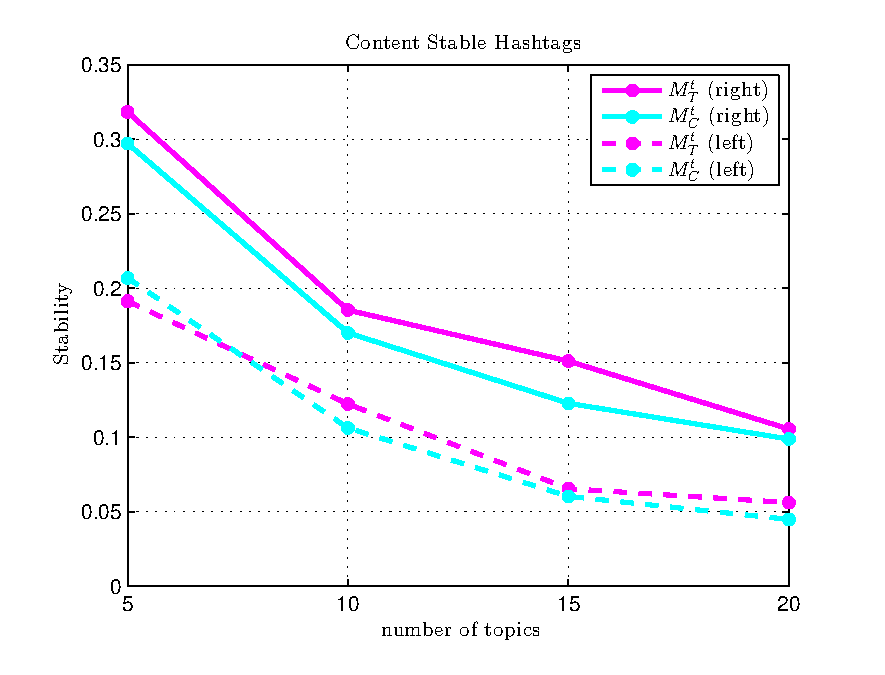
\includegraphics[width=\textwidth]{KDD/images/content_stable_eigen_left_right}          
	%{\tiny(a) Content Stable }
\end{minipage} 
\begin{minipage}{0.49\linewidth}
  \centering
  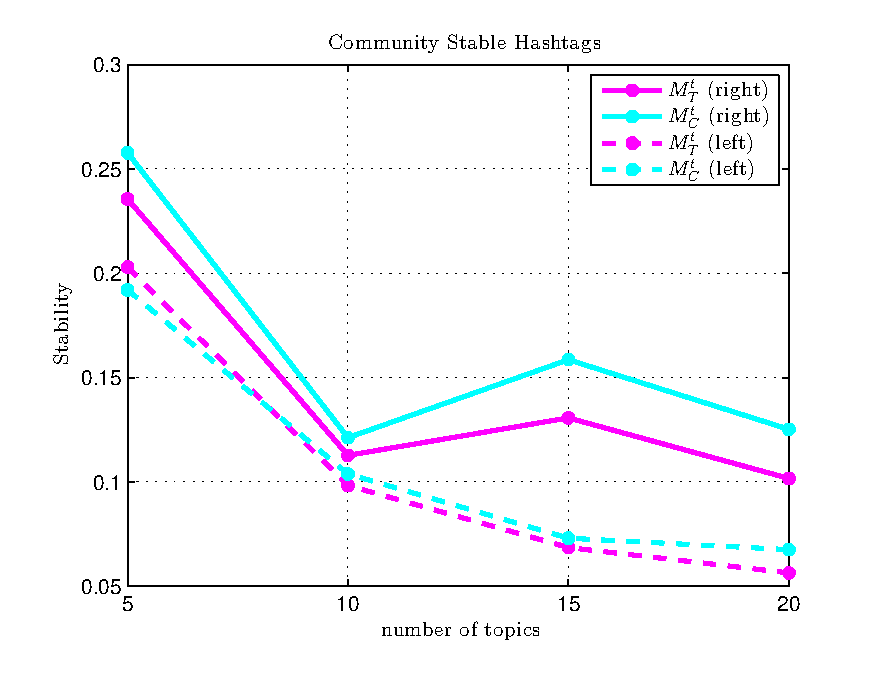
\includegraphics[width=\textwidth]{KDD/images/community_stable_eigen_left_right}             
	%{\tiny(b) Community Stable}
\end{minipage} 
  \caption[Stability of evolution matrices]{{This figure plots the stability of $\MC$ and $\MT$.
We note that in (a) $\MT$ matrix shows higher stability than the $\MC$ matrix,
and in (b) $\MC$ shows higher stability than $\MC$, thus confirming that we are indeed able to learn the 
stability through our algorithm.}}
  \label{fig:stability_analysis}
}
\end{center}
\end{figure*}
